% \subsection{Jednocestný usměrňovač}

\begin{figure}[h!]
    \centering
    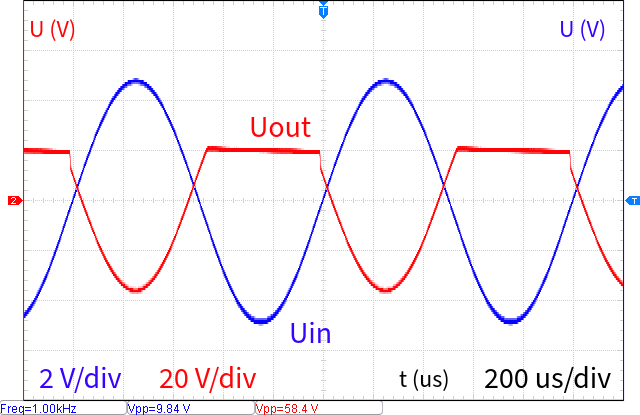
\includegraphics[width=0.8\textwidth]{lab/output3.png}
    \caption{Zapojení a) -- Časová závislost napětí na kondenzátoru (modře) a na výstupu OZ (červeně), \(R_{p} =\qty{100}{\kilo\ohm}\).}
    \label{fig:lab/output3.png}
\end{figure}

\begin{figure}[h!]
    \centering
    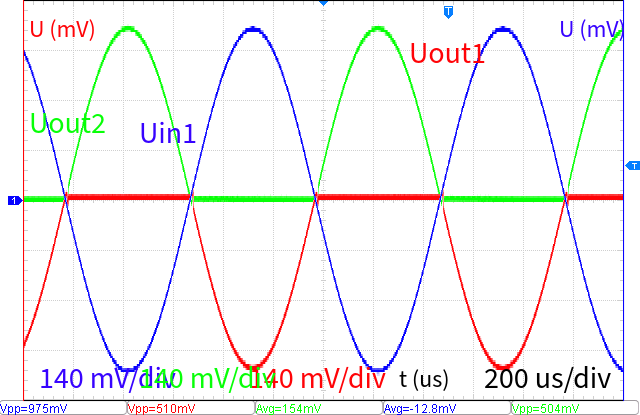
\includegraphics[width=0.8\textwidth]{lab/output1.png}
    \caption{Zapojení a) -- Stejně jako v Obr. \ref{fig:lab/output3.png}, ale pro \(R_{p} =\qty{0}{\ohm}\), je patrné zkreslení dané mezní rychlostí přeběhu.}
    \label{fig:lab/output1.png}
\end{figure}

\begin{figure}[h!]
    \centering
    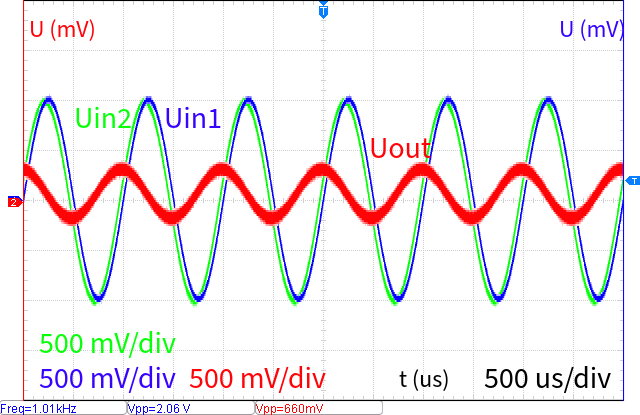
\includegraphics[width=0.8\textwidth]{lab/output6.png}
    \caption{Zapojení b) -- Časová závislost napětí na výstupu prvního OZ (obdélník) a druhého OZ (pila), \(R_{p} =\qty{100}{\kilo\ohm}\).}
    \label{fig:lab/output6.png}
\end{figure}

\begin{figure}[h!]
    \centering
    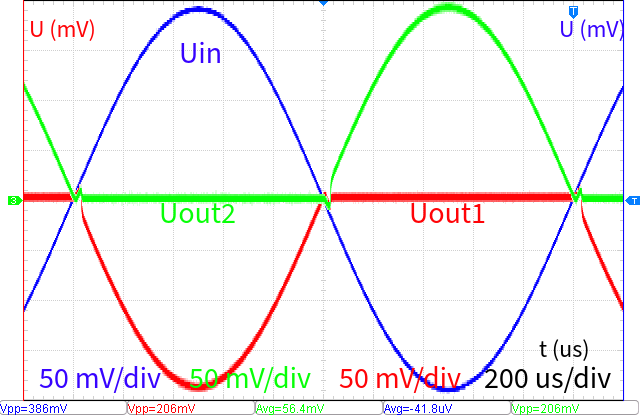
\includegraphics[width=0.8\textwidth]{lab/output4.png}
    \caption{Zapojení b) -- Stejě jako v Obr. \ref{fig:lab/output6.png}, ale pro \(R_{p} =\qty{0}{\ohm}\), opět na této frekvenci vidíme zkosení hran dané nedostatečnou hodnotou SR u tohoto OZ.}
    \label{fig:lab/output4.png}
\end{figure}



\begin{table}[]
    \caption{Porovnání strmostí v simulaci a laboratoři.}
    \centering
    \def\arraystretch{1.4}
    \begin{tabular}{l|l|l|l||l|l|l}
        & \multicolumn{2}{l|}{Zap a) sim} & Zap a) lab & \multicolumn{2}{l|}{Zap b) sim} & Zap b) lab \\ \hline
    typ OZ             & 1458       & 072   & 1458       & 1458       & 072   & 1458       \\ \hline
    \(f_{min} \)  [Hz]      & 100        &   100   & 89         & 108        &    108  & 98         \\ \hline
    \(f_{max} \)  [Hz]      & 8000       &   8000   & 6860       & 7634       &    7634  & 6340       \\ \hline
    S [V/\unit{\micro\second}] & 0,44       & 4,63 & 0,61       & 0,48       & 6,77 & 0,61      
    \end{tabular}
    \label{tab:tabulka_hodnot_brewster}
    \end{table}